\documentclass{article}
\usepackage{amsmath}
\usepackage{tikz}
\usepackage{pgfplots}

\pgfplotsset{compat=1.17}

\begin{document}

\title{Understanding\\the Slope-Intercept Form\\of Linear Equations}\\
\author{Tutoring Centre Ferndale\\
\includegraphics[width=4em]{ApS_logo.png}}
\date{}
\maketitle

In linear algebra, the slope-intercept form of a linear equation is a straightforward and intuitive way to represent a line.

\section*{Slope-Intercept Form: \( y = mx + b \)}

In the slope-intercept form,
\begin{itemize}
    \item \( m \) is the slope of the line.
    \item \( b \) is the y-intercept, the point where the line crosses the y-axis.
\end{itemize}

\section*{Converting Standard Form to Slope-Intercept Form}

To convert a linear equation from standard form \( Ax + By = C \) to slope-intercept form \( y = mx + b \):

\[
Ax + By = C
\]
\[
By = -Ax + C
\]
\[
y = -\frac{A}{B}x + \frac{C}{B}
\]

Here, the slope \( m \) is \(-\frac{A}{B}\), and the y-intercept \( b \) is \(\frac{C}{B}\).

\newpage

\section*{Calculating the Slope \( m \)}

The slope \( m \) is calculated using the change in $x$ and the change in $y$ between two points on the line.\\

The mathematical symbol for change is the Greek letter $\Delta$ delta, equivalent to the English letter D, standing for "difference."\\

\begin{center}
Thus, $m=\frac{\Delta x}{\Delta y}$\\
\end{center}

These are also known as the rise and the run.

\begin{itemize}
    \item The rise is the change in the y-coordinate.
    \item The run is the change in the x-coordinate.
\end{itemize}

\[
m = \frac{\Delta x}{\Delta y} = \frac{\text{rise}}{\text{run}} = \frac{y_2 - y_1}{x_2 - x_1}
\]

\subsection*{Example}

Consider two points \((1, 2)\) and \((4, 5)\). The slope \( m \) is calculated as follows:

\[
m = \frac{5 - 2}{4 - 1} = \frac{3}{3} = 1
\]

\begin{center}
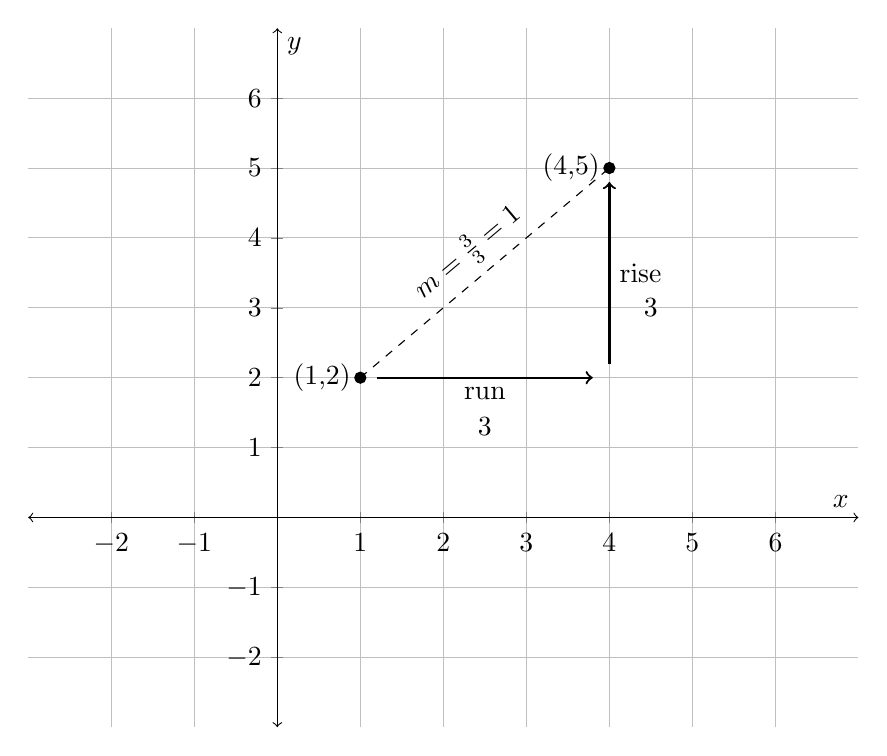
\begin{tikzpicture}
    \begin{axis}[width=\textwidth,
                 axis lines=middle,
                 axis line style={<->},
                 xlabel={$x$},
                 ylabel={$y$},
                 xmin=-3, xmax=7,
                 ymin=-3, ymax=7,
                 xtick={-2,-1,...,6},
                 ytick={-2,-1,...,6},
                 grid=both,
                 grid style={line width=.3pt, draw=gray!50}]
    \addplot[only marks, mark=*]
    coordinates {(1,2) (4,5)};
    \node at (axis cs:1,2) [anchor=east] {(1,2)};
    \node at (axis cs:4,5) [anchor=east] {(4,5)};
    \draw[->, thick] (axis cs:1.2,2) -- (axis cs:3.8,2) node[midway, below] {run};
    \draw[->, thick] (axis cs:4,2.2) -- (axis cs:4,4.8) node[midway, right] {rise};
    \node at (axis cs:2.5,1.3) {3};
    \node at (axis cs:4.5,3) {3};
    \draw[dashed] (axis cs:1,2) -- (axis cs:4,5) node[pos=0.5, sloped, above] {$m=\frac{3}{3}=1$};
    \end{axis}
\end{tikzpicture}
\end{center}

\newpage

\section*{Effect of Changing the Slope \( m \)}

\begin{itemize}
    \item \( m \) determines the steepness and direction of the line.
    \item A positive \( m \) results in an upward-sloping line, while a negative \( m \) results in a downward-sloping line.
    \item The larger the absolute value of \( m \), the steeper the line.
\end{itemize}

\paragraph{Absolute Value:}
The absolute value of a number is its distance from zero on the number line, regardless of direction. It is always a non-negative number. Any negative sign is stripped away, making the result positive or zero. The absolute value of a number \(x\) is denoted by \(|x|\).\\

\subsection*{Example}



The graph shows three lines with different slopes: \( y = x + 1 \), \( y = 2x + 1 \), and \( y = -x + 1 \). The slope \( m \) affects the steepness and direction of the lines.

\newpage

\section*{Effect of Changing the y-intercept \( b \)}

\begin{itemize}
    \item \( b \) determines the point where the line crosses the y-axis.
    \item Changing \( b \) shifts the line up or down without altering its slope.
\end{itemize}

\subsection*{Example}

\begin{center}
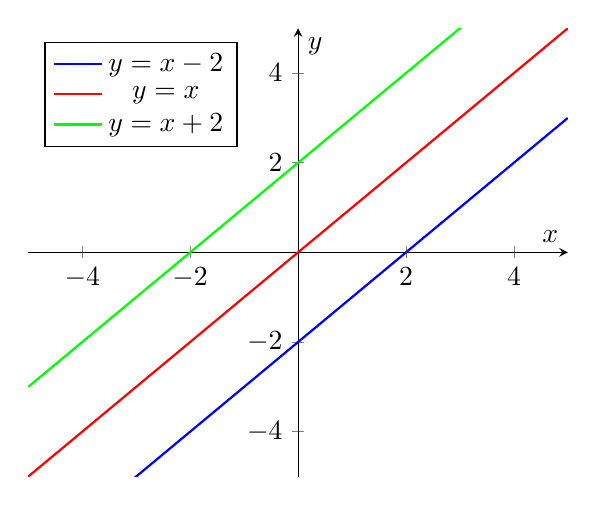
\begin{tikzpicture}
    \begin{axis}[
        axis lines = middle,
        xlabel = {$x$},
        ylabel = {$y$},
        ymin=-5, ymax=5,
        xmin=-5, xmax=5,
        domain=-5:5,
        samples=100,
        legend pos=north west
    ]
    \addplot [blue, thick] {1*x - 2};
    \addplot [red, thick] {1*x + 0};
    \addplot [green, thick] {1*x + 2};
    \legend{$y = x - 2$, $y = x$, $y = x + 2$}
    \end{axis}
\end{tikzpicture}
\end{center}

The graph shows three lines with different y-intercepts: \( y = x - 2 \), \( y = x \), and \( y = x + 2 \). The y-intercept \( b \) affects the vertical position of the lines.

\newpage

\section*{Plotting the Graph Using Slope and $y$-intercept}

To plot a line using the slope-intercept form:
\begin{itemize}
    \item Start at the y-intercept \((0, b)\).
    \item Use the slope \( m \) to determine the rise and run from the y-intercept.
    \item Plot additional points using the rise and run and draw the line through these points.
\end{itemize}

\subsection*{Example}

For the equation \( y = 2x + 1 \):
\begin{itemize}
    \item Start at the y-intercept \((0, 1)\).
    \item Use the slope \( m = 2 \) to plot the next point: rise = 2, run = 1, leading to point \((1, 3)\).
    \item Draw the line through these points.
\end{itemize}

\begin{center}
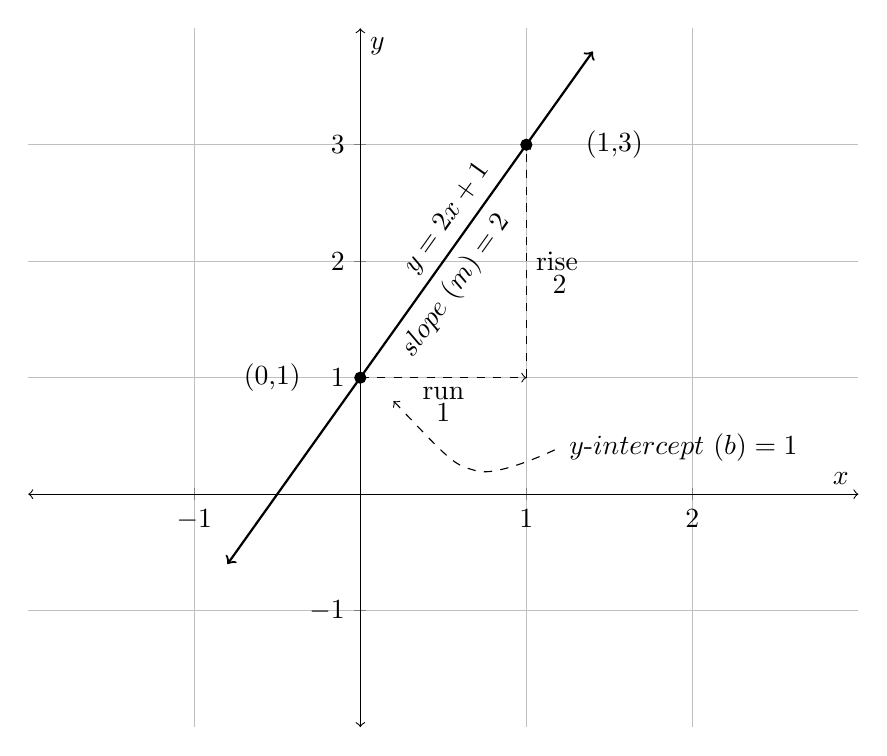
\begin{tikzpicture}
    \begin{axis}[width=\textwidth,
                 axis lines=middle,
                 axis line style={<->},
                 xlabel={$x$},
                 ylabel={$y$},
                 xmin=-2, xmax=3,
                 ymin=-2, ymax=4,
                 xtick={-1,0,1,2},
                 ytick={-1,0,1,2,3},
                 grid=both,
                 grid style={line width=.3pt, draw=gray!50}]
    \addplot[only marks, mark=*]
    coordinates {(0,1) (1,3)};
    \node at (axis cs:-0.3,1) [anchor=east] {(0,1)};
    \node at (axis cs:1.3,3) [anchor=west] {(1,3)};
    \draw[->, dashed] (axis cs:0,1) -- (axis cs:1,1) node[midway, below] {run};
    \draw[->, dashed] (axis cs:1,1) -- (axis cs:1,3) node[midway, right] {rise};
    \node at (axis cs:0.5,0.7) {1};
    \node at (axis cs:1.2,1.8) {2};
    \draw[thick,<->] (axis cs:-.8,-.6) -- (axis cs:1.4,3.8) node[pos=0.57, sloped, below] {$slope \ (m)=2$} node[pos=0.65, sloped, above]{$y=2x+1$};
    \draw[<-,dashed] plot [smooth] coordinates {(axis cs:.2,.8) (axis cs:.7,0.2) (axis cs:1.2,.4)} node[right] {$y\text{-}intercept \ (b)=1$};
    \end{axis}
\end{tikzpicture}
\end{center}

\newpage

\section*{Real-Life Examples}

\subsection*{Example 1: Budgeting}

Suppose you earn a fixed amount of money each week, and you have some initial savings. The total amount of money you have after \( x \) weeks can be modeled by a linear equation.

\[
y = mx + b
\]

Where:
\begin{itemize}
    \item \( m \) is the weekly earnings.
    \item \( b \) is the initial savings.
\end{itemize}

\subsection*{Example 2: Distance Over Time}

Suppose you are traveling at a constant speed. The distance traveled after \( x \) hours can be modeled by a linear equation.

\[
y = mx + b
\]

Where:
\begin{itemize}
    \item \( m \) is the speed.
    \item \( b \) is the initial distance (if any).
\end{itemize}

\newpage

\section*{Practice Questions}

\begin{enumerate}
    \item Find the slope and y-intercept of the line given by the equation \( y = 3x - 4 \).
    \item Convert the standard form equation \( 2x + 3y = 6 \) to slope-intercept form and identify the slope and y-intercept.
    \item Write the equation of a line with a slope of 2 and a y-intercept of -3.
    \item A person saves \$50 each week starting with \$200. Write the equation representing the total savings after \( x \) weeks.
    \item For the equation \( y = -\frac{1}{2}x + 4 \), plot the graph and determine the coordinates of two points on the line.
\end{enumerate}

\section*{Answers}

\begin{enumerate}
    \item Slope \( m = 3 \), y-intercept \( b = -4 \).
    \item \( y = -\frac{2}{3}x + 2 \). Slope \( m = -\frac{2}{3} \), y-intercept \( b = 2 \).
    \item \( y = 2x - 3 \).
    \item \( y = 50x + 200 \).
    \item Two points on the line: \((0, 4)\) and \((2, 3)\):
\end{enumerate}

\begin{center}
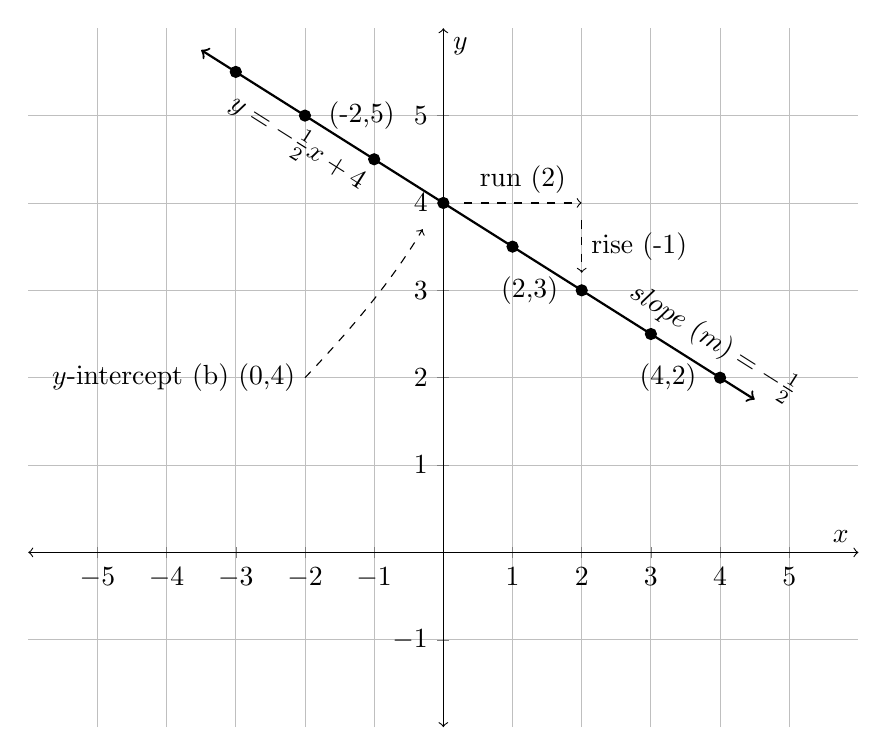
\begin{tikzpicture}
    \begin{axis}[width=\textwidth,
                 axis lines=middle,
                 axis line style={<->},
                 xlabel={$x$},
                 ylabel={$y$},
                 xmin=-6, xmax=6,
                 ymin=-2, ymax=6,
                 xtick={-5,-4,...,5},
                 ytick={-1,0,...,5},
                 grid=both,
                 grid style={line width=.3pt, draw=gray!50}]
    \addplot[only marks, mark=*]
    coordinates {(-3,5.5) (-2,5) (-1,4.5) (0,4) (1,3.5) (2,3) (3,2.5) (4,2)};
    \node at (axis cs:-1.8,5) [anchor=west] {(-2,5)};
    \node at (axis cs:1.8,3) [anchor=east] {(2,3)};
    \node at (axis cs:3.8,2) [anchor=east] {(4,2)};
    \draw[->, dashed] (axis cs:0.3,4) -- (axis cs:2,4) node[midway, above] {run (2)};
    \draw[->, dashed] (axis cs:2,3.8) -- (axis cs:2,3.2) node[midway, right] {rise (-1)};
    \draw[thick,<->] (axis cs:-3.5,5.75) -- (axis cs:4.5,1.75)
        node[pos=0.9, sloped, above] {$slope \ (m)=-\frac{1}{2}$}
        node[pos=0.2, sloped, below]{$y=-\frac{1}{2}x+4$};
    \node at (axis cs:-2,2) [anchor=east] {$y$-intercept (b) (0,4)};
    \draw[->, dashed] plot [smooth, tension=1] coordinates {(-2,2) (-1,2.9) (-0.3,3.7)};
    \end{axis}
\end{tikzpicture}
\end{center}

\end{document}
